\documentclass[a4paper, 14pt]{extarticle}

% Поля
%--------------------------------------
\usepackage{geometry}
\geometry{a4paper,tmargin=2cm,bmargin=2cm,lmargin=3cm,rmargin=1cm}
%--------------------------------------


%Russian-specific packages
%--------------------------------------
\usepackage[T2A]{fontenc}
\usepackage[utf8]{inputenc} 
\usepackage[english, main=russian]{babel}
%--------------------------------------

\usepackage{textcomp}

% Красная строка
%--------------------------------------
\usepackage{indentfirst}               
%--------------------------------------             


%Graphics
%--------------------------------------
\usepackage{graphicx}
\graphicspath{ {./images/} }
\usepackage{wrapfig}
%--------------------------------------

% Полуторный интервал
%--------------------------------------
\linespread{1.3}                    
%--------------------------------------

%Выравнивание и переносы
%--------------------------------------
% Избавляемся от переполнений
\sloppy
% Запрещаем разрыв страницы после первой строки абзаца
\clubpenalty=10000
% Запрещаем разрыв страницы после последней строки абзаца
\widowpenalty=10000
%--------------------------------------

%Списки
\usepackage{enumitem}

%Подписи
\usepackage{caption} 

%Гиперссылки
\usepackage{hyperref}

\hypersetup {
	unicode=true
}

%Рисунки
%--------------------------------------
\DeclareCaptionLabelSeparator*{emdash}{~--- }
\captionsetup[figure]{labelsep=emdash,font=onehalfspacing,position=bottom}
%--------------------------------------

\usepackage{tempora}
\usepackage{amsmath}
\usepackage{color}
\usepackage{listings}
\lstset{
  belowcaptionskip=1\baselineskip,
  breaklines=true,
  frame=L,
  xleftmargin=\parindent,
  language=Java,
  showstringspaces=false,
  basicstyle=\footnotesize\ttfamily,
  keywordstyle=\bfseries\color{blue},
  commentstyle=\itshape\color{purple},
  identifierstyle=\color{black},
  stringstyle=\color{red},
}

%--------------------------------------
%			НАЧАЛО ДОКУМЕНТА
%--------------------------------------

\begin{document}

%--------------------------------------
%			ТИТУЛЬНЫЙ ЛИСТ
%--------------------------------------
\begin{titlepage}
\thispagestyle{empty}
\newpage


%Шапка титульного листа
%--------------------------------------
\vspace*{-60pt}
\hspace{-65pt}
\begin{minipage}{0.3\textwidth}
\hspace*{-20pt}\centering

\includegraphics[width=\textwidth]{emblem}
\end{minipage}
\begin{minipage}{0.67\textwidth}\small \textbf{
\vspace*{-0.7ex}
\hspace*{-6pt}\centerline{Министерство науки и высшего образования Российской Федерации}
\vspace*{-0.7ex}
\centerline{Федеральное государственное бюджетное образовательное учреждение }
\vspace*{-0.7ex}
\centerline{высшего образования}
\vspace*{-0.7ex}
\centerline{<<Московский государственный технический университет}
\vspace*{-0.7ex}
\centerline{имени Н.Э. Баумана}
\vspace*{-0.7ex}
\centerline{(национальный исследовательский университет)>>}
\vspace*{-0.7ex}
\centerline{(МГТУ им. Н.Э. Баумана)}}
\end{minipage}
%--------------------------------------

%Полосы
%--------------------------------------
\vspace{-25pt}
\hspace{-35pt}\rule{\textwidth}{2.3pt}

\vspace*{-20.3pt}
\hspace{-35pt}\rule{\textwidth}{0.4pt}
%--------------------------------------

\vspace{1.5ex}
\hspace{-35pt} \noindent \small ФАКУЛЬТЕТ\hspace{80pt} <<Информатика и системы управления>>

\vspace*{-16pt}
\hspace{47pt}\rule{0.83\textwidth}{0.4pt}

\vspace{0.5ex}
\hspace{-35pt} \noindent \small КАФЕДРА\hspace{50pt} <<Теоретическая информатика и компьютерные технологии>>

\vspace*{-16pt}
\hspace{30pt}\rule{0.866\textwidth}{0.4pt}
  
\vspace{11em}

\begin{center}
\Large {\bf Летучка № 2} \\ 
\large {\bf по курсу <<Языки и методы программирования>>} \\ 
\large <<Создание "обертки" для веб-сервера>>
\end{center}\normalsize

\vspace{8em}


\begin{flushright}
  {Студент группы ИУ9-21Б Воронков А. С.\hspace*{15pt} \\
  \vspace{2ex}
  Преподаватель Посевин Д. П.\hspace*{15pt}}
\end{flushright}

\bigskip

\vfill
 

\begin{center}
\textsl{Москва 2026}
\end{center}
\end{titlepage}
%--------------------------------------
%		КОНЕЦ ТИТУЛЬНОГО ЛИСТА
%--------------------------------------

\renewcommand{\ttdefault}{pcr}

\setlength{\tabcolsep}{3pt}
\newpage
\setcounter{page}{2}

\section{Цель}\label{Sect::task}
\par
Преобразовать "обертку"  для веб-сервера согласно индивидиальному варианту

\section{Индивидуальный вариант}
\par 
Реализовать "обертку" веб-сервера для следующих классов:
\begin{enumerate}
    \item Класс HTTP-кодов и сообщений об ошибках
    \item Класс $n$-мерных векторов
\end{enumerate}
\pagebreak
\section{Практическая реализация}
Код файла Test1.java
\begin{lstlisting}
import java.io.IOException;
import java.io.OutputStream;
import java.net.InetSocketAddress;
import java.net.URLDecoder;
import java.nio.charset.StandardCharsets;
import java.util.HashMap;
import java.util.Map;

import com.sun.net.httpserver.HttpExchange;
import com.sun.net.httpserver.HttpHandler;
import com.sun.net.httpserver.HttpServer;

class HttpStatusCode {
    private final String reason;
    private final int code;

    HttpStatusCode(String reason, int code) {
        this.reason = reason;
        this.code = code;
    }

    String getReason() {
        return reason;
    }

    int getCode() {
        return code;
    }
}

class QueryParser {

    static Map<String, String> parse(String query) {
        Map<String, String> params = new HashMap<>();
        if (query == null || query.isEmpty())
            return params;

        for (String pair : query.split("&")) {
            String[] parts = pair.split("=", 2);
            if (parts.length != 2)
                continue;

            String key = URLDecoder.decode(parts[0], StandardCharsets.UTF_8);
            String value = URLDecoder.decode(parts[1], StandardCharsets.UTF_8);
            params.put(key, value);
        }
        return params;
    }
}

class HttpStatusCodeMapper {

    static HttpStatusCode fromParams(Map<String, String> params) {
        String reason = params.getOrDefault("reason", "Ok");
        int code = Integer.parseInt(params.getOrDefault("code", "200"));
        return new HttpStatusCode(reason, code);
    }
}

class PersonJsonSerializer {

    static String toJson(HttpStatusCode p) {
        int id = System.identityHashCode(p);

        return """
        {
          "code": "%d",
          "reason": %s,
          "objectId": "%s"
        }
        """.formatted(
                p.getCode(),
                escape(p.getReason()),
                Integer.toHexString(id));
    }

    private static String escape(String s) {
        return s.replace("\"", "\\\"");
    }
}

public class Test1 {

    public static void main(String[] args) throws Exception {
        HttpServer server = HttpServer.create(new InetSocketAddress(5678), 0);
        server.createContext("/test", new MyHandler());
        server.setExecutor(null); // creates a default executor
        server.start();
    }

    static class MyHandler implements HttpHandler {
        @Override
        public void handle(HttpExchange exchange) throws IOException {
            if (!"GET".equals(exchange.getRequestMethod())) {
                exchange.sendResponseHeaders(405, -1);
                return;
            }

            String query = exchange.getRequestURI().getQuery();
            Map<String, String> params = QueryParser.parse(query);

            HttpStatusCode person;
            try {
                person = HttpStatusCodeMapper.fromParams(params);
            } catch (NumberFormatException e) {
                exchange.sendResponseHeaders(400, -1);
                return;
            }

            String json = PersonJsonSerializer.toJson(person);

            exchange.getResponseHeaders().add("Content-Type", "application/json");
            exchange.sendResponseHeaders(200, json.getBytes().length);

            try (OutputStream os = exchange.getResponseBody()) {
                os.write(json.getBytes());
            }
        }
    }
}
\end{lstlisting}
\par
Код файла Test2.java
\begin{lstlisting}
import java.io.IOException;
import java.io.OutputStream;
import java.net.InetSocketAddress;
import java.net.URLDecoder;
import java.nio.charset.StandardCharsets;
import java.util.HashMap;
import java.util.Map;

import com.sun.net.httpserver.HttpExchange;
import com.sun.net.httpserver.HttpHandler;
import com.sun.net.httpserver.HttpServer;

class Vector {
    private final String vector;

    Vector(String vector) {
        this.vector = vector;
    }

    String getVector() {
        return vector;
    }
}

class QueryParser {

    static Map<String, String> parse(String query) {
        Map<String, String> params = new HashMap<>();
        if (query == null || query.isEmpty())
            return params;

        for (String pair : query.split("&")) {
            String[] parts = pair.split("=", 2);
            if (parts.length != 2)
                continue;

            String key = URLDecoder.decode(parts[0], StandardCharsets.UTF_8);
            String value = URLDecoder.decode(parts[1], StandardCharsets.UTF_8);
            params.merge(key, value, (oldVal, newVal) -> oldVal + ", " + newVal);
        }
        return params;
    }
}

class VectorMapper {

    static Vector fromParams(Map<String, String> params) {
        String reason = params.getOrDefault("vector", "0");
        return new Vector(reason);
    }
}

class VectorJsonSerializer {

    static String toJson(Vector p) {
        int id = System.identityHashCode(p);

        return """
        {
          "vector": "(%s)",
          "objectId": "%s"
        }
        """.formatted(
                p.getVector(),
                Integer.toHexString(id));
    }

    private static String escape(String s) {
        return s.replace("\"", "\\\"");
    }
}

public class Test2 {

    public static void main(String[] args) throws Exception {
        HttpServer server = HttpServer.create(new InetSocketAddress(5678), 0);
        server.createContext("/test", new MyHandler());
        server.setExecutor(null); // creates a default executor
        server.start();
    }

    static class MyHandler implements HttpHandler {
        @Override
        public void handle(HttpExchange exchange) throws IOException {
            if (!"GET".equals(exchange.getRequestMethod())) {
                exchange.sendResponseHeaders(405, -1);
                return;
            }

            String query = exchange.getRequestURI().getQuery();
            Map<String, String> params = QueryParser.parse(query);

            Vector vector;
            try {vector = VectorMapper.fromParams(params);
            } catch (NumberFormatException e) {
                exchange.sendResponseHeaders(400, -1);
                return;
            }

            String json = VectorJsonSerializer.toJson(vector);

            exchange.getResponseHeaders().add("Content-Type", "application/json");
            exchange.sendResponseHeaders(200, json.getBytes().length);

            try (OutputStream os = exchange.getResponseBody()) {
                os.write(json.getBytes());
            }
        }
    }
}
\end{lstlisting}

\section{Результаты}
В результате работы программы получилось запустить "обертки" на веб-серверах для двух классов. Класс HTTP кодов выводит код ошибки, причину и айди объекта. Класс векторов выводит строку координат вектора и айди объекта.

\begin{center}
    \nopagebreak
    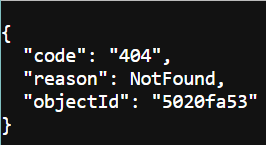
\includegraphics[width=0.85\textwidth]{s1}
    \captionsetup{justification=centering}
    \captionof{figure}{Результат запроса с параметрами ошибки: \\ \url{http://185.102.139.168:5678/test?code=404&reason=NotFound}}

    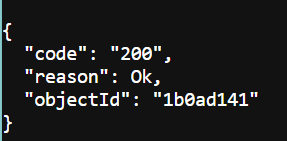
\includegraphics[width=0.85\textwidth]{s2}
    \captionsetup{justification=centering}
    \captionof{figure}{Результат запроса без параметров ошибки: \\ \url{http://185.102.139.168:5678/test}}

    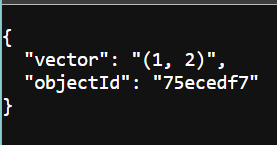
\includegraphics[width=0.85\textwidth]{s3}
    \captionsetup{justification=centering}
    \captionof{figure}{Результат запроса с параметрами вектора: \\ \url{http://185.102.139.168:5678/test?vector=1&vector=2}}

    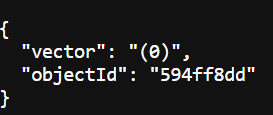
\includegraphics[width=0.85\textwidth]{s4}
    \captionsetup{justification=centering}
    \captionof{figure}{Результат запроса без параметров вектора: \\ \url{http://185.102.139.168:5678/test}}
\end{center}

\section{Вывод}
В данной лабораторной работе была изменена "обертка" и переработана под новые классы. Изначальный код был разобран и преобразован под требуемое задание.
\end{document}